\documentclass[10pt,a4paper]{article}
\usepackage[utf8]{inputenc}
\usepackage{amsmath}
\usepackage{amsfonts}
\usepackage{amssymb}
\usepackage{graphicx}
\usepackage{sectsty}
\allsectionsfont{\centering} 
\begin{document}
%-----------------------------------------------------------------------------------------------------
\section*{Front End}
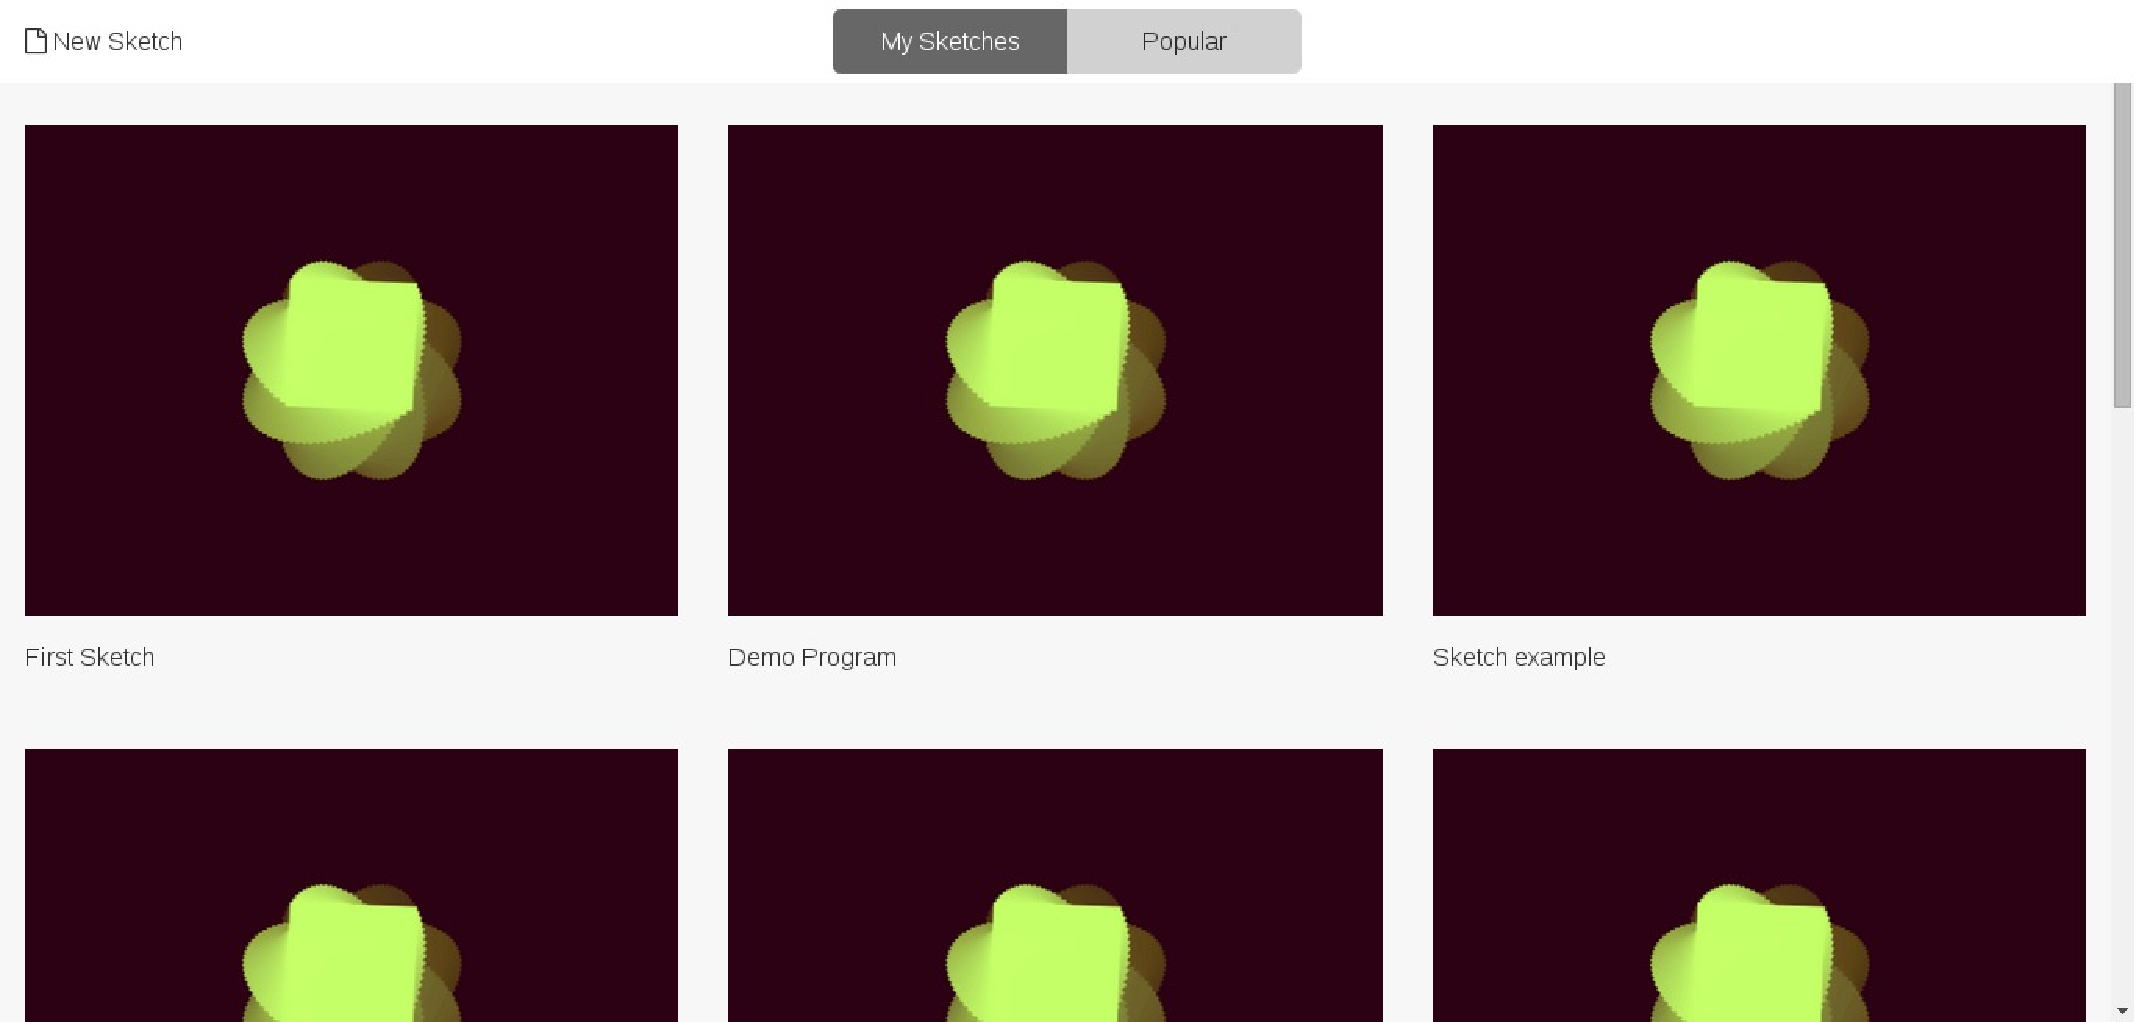
\includegraphics[width=\textwidth,keepaspectratio]{browser.pdf}
\hfill\\
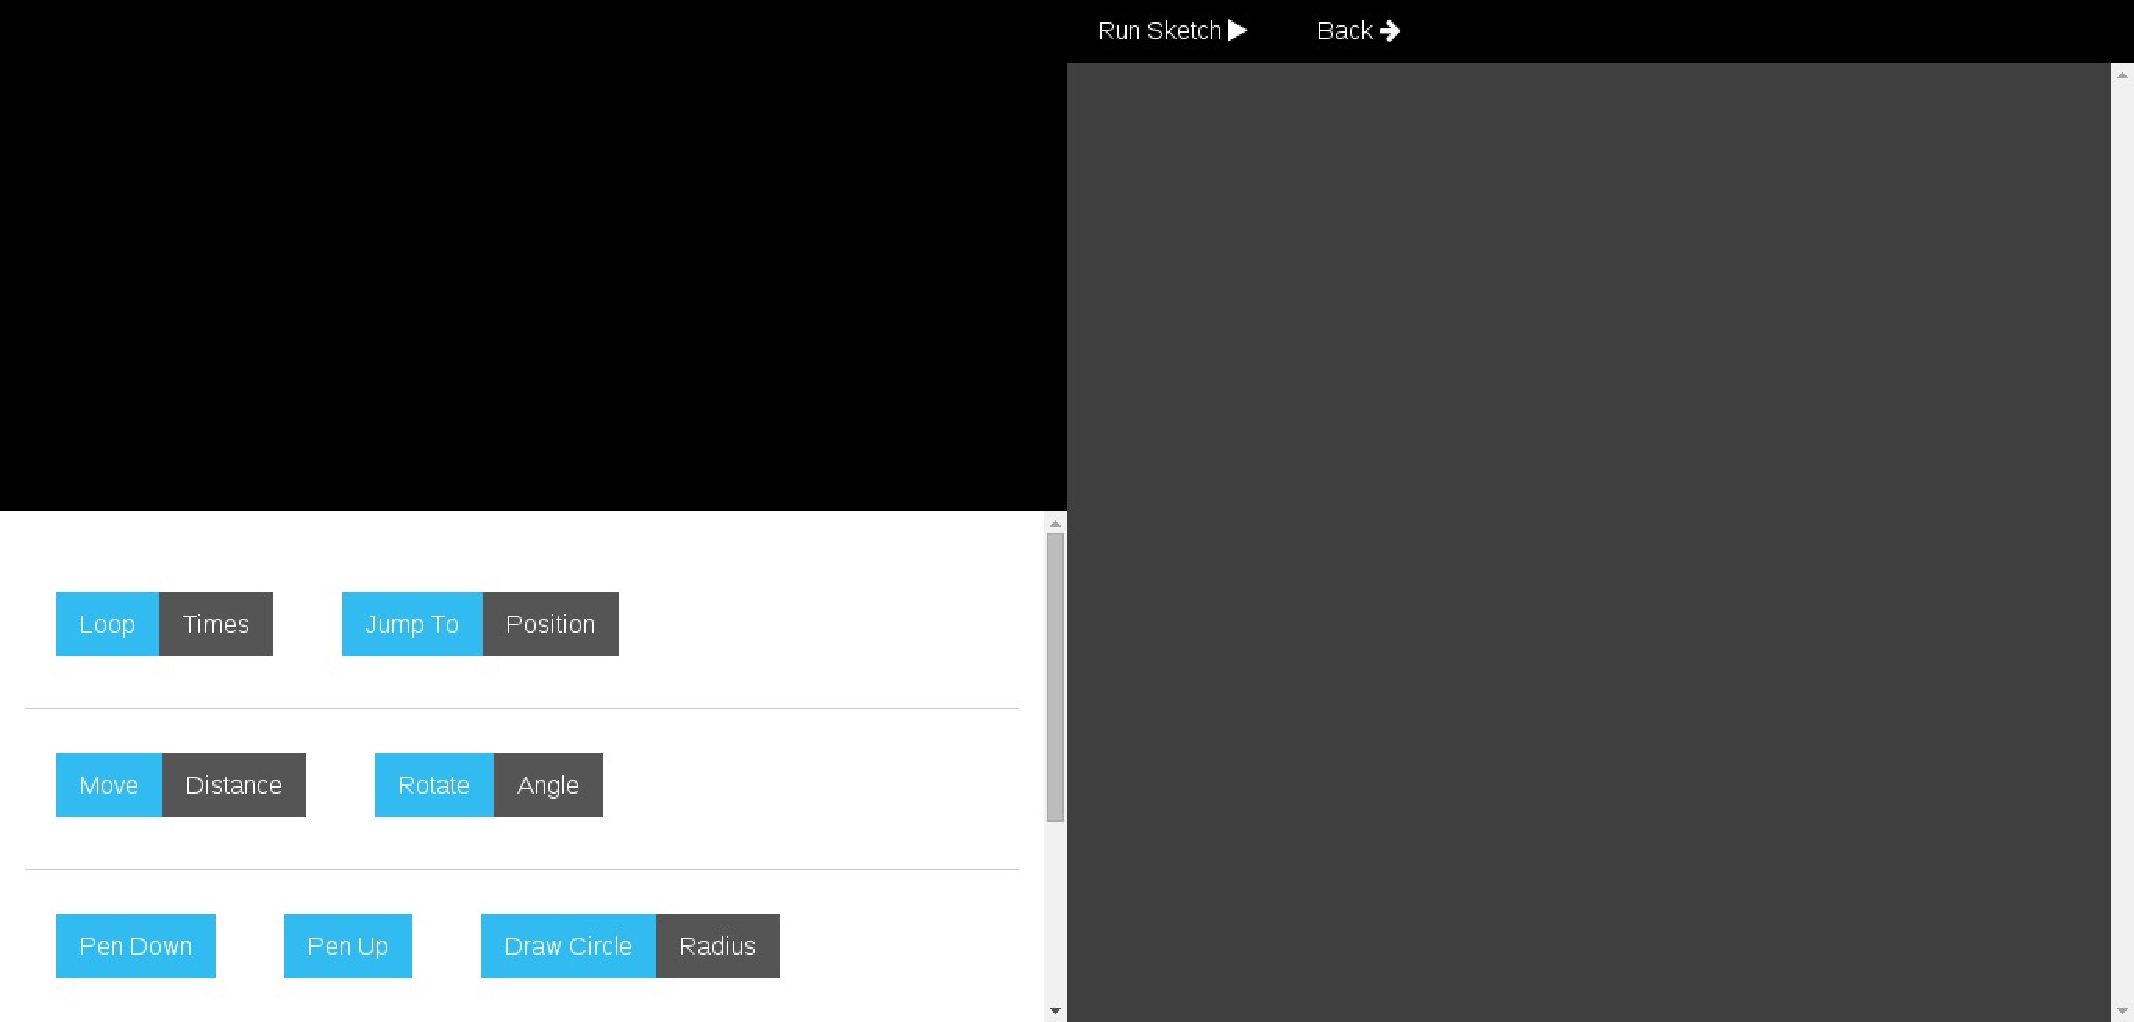
\includegraphics[width=\textwidth,keepaspectratio]{editor.pdf}
\hfill\\
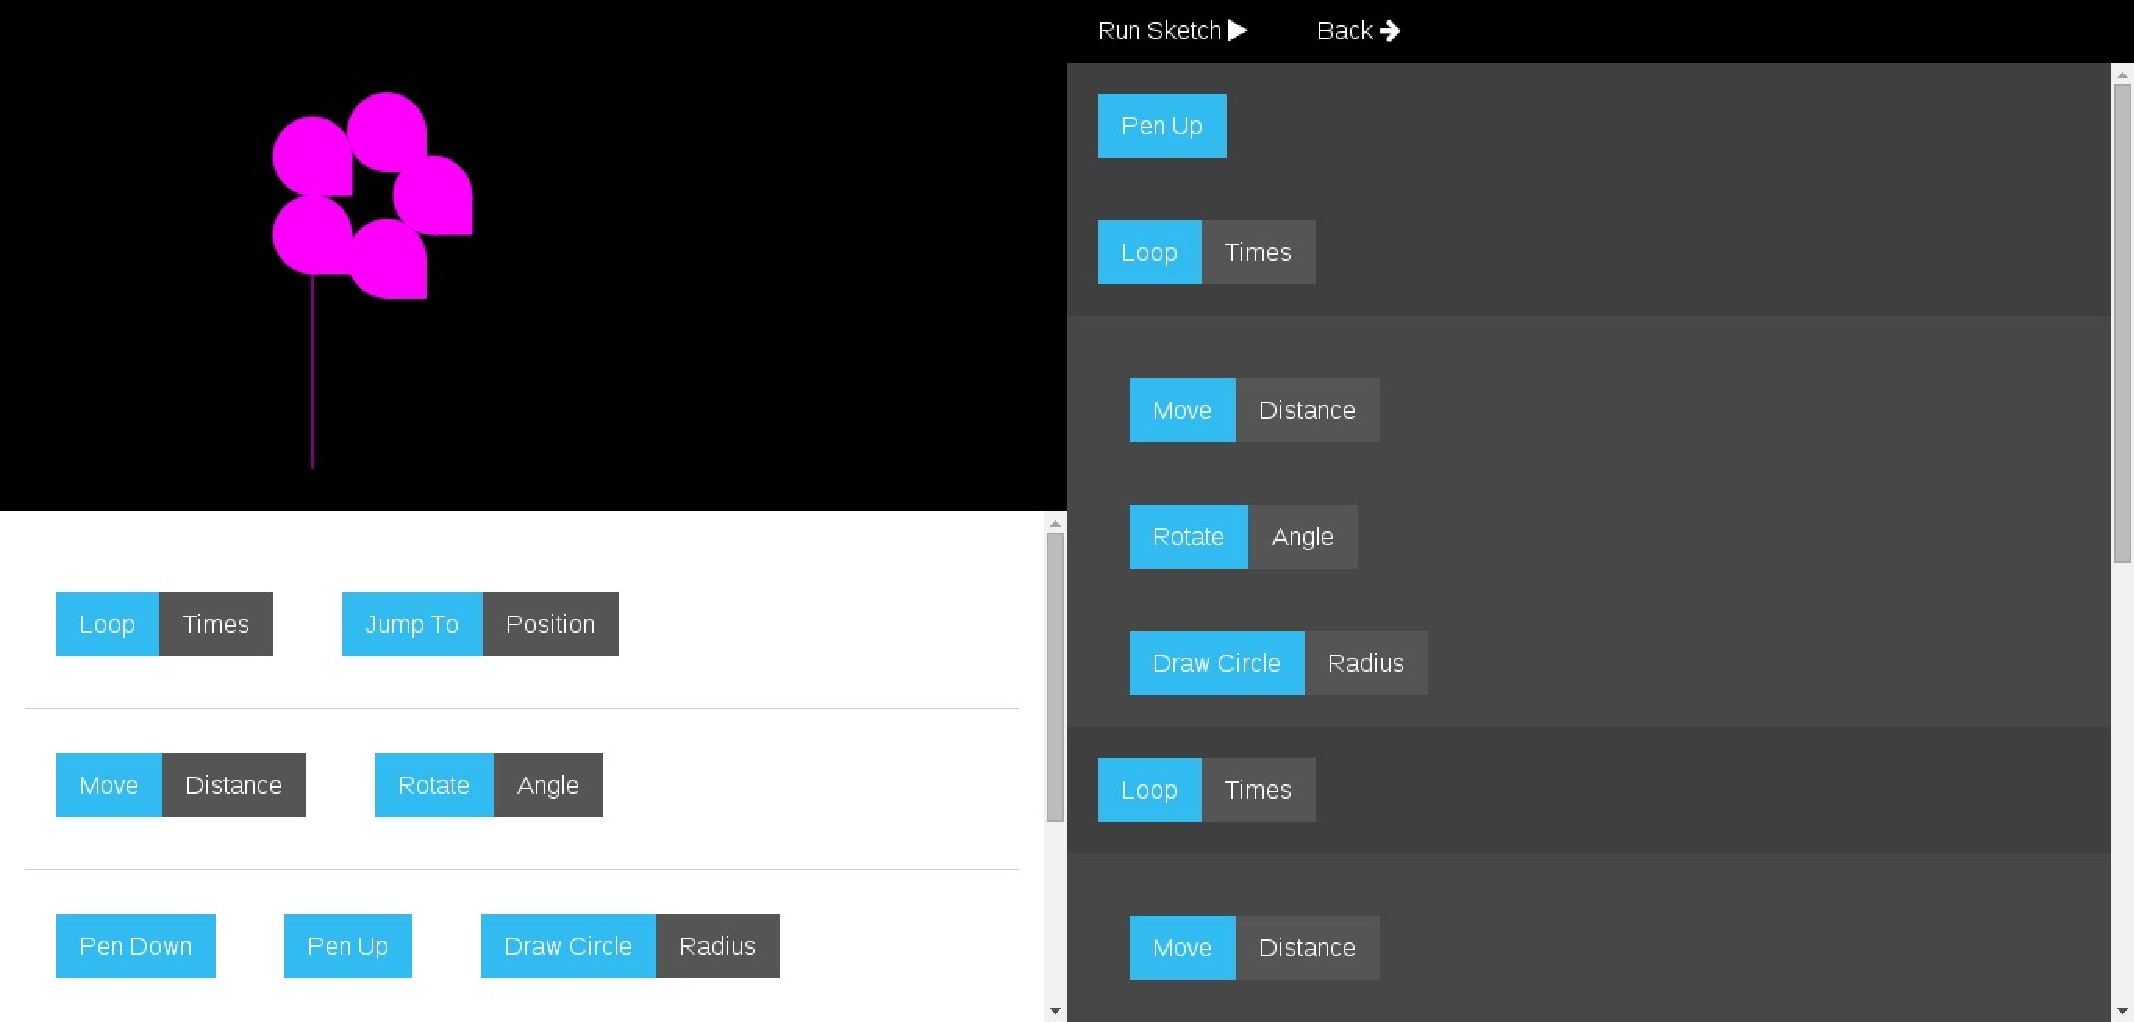
\includegraphics[width=\textwidth,keepaspectratio]{editor_with_contents.pdf}
%-----------------------------------------------------------------------------------------------------
\newpage
\section*{System Architecture.}
\begin{itemize}
\item Hosted on heroku.
\item Logical teir is nodejs.
\item Data teir is Postgres.
\item Preview images stored on s3
\end{itemize}
%----------------------------------------------------------------------------------------------------
\newpage
\section*{Scalability.}
		\begin{itemize}
		\item Stateless protocol.
		\item Client side computation.
		\begin{itemize}
		\item Images are encoded on the client side.
		\end{itemize}				
		\item Caching.
		\begin{itemize}
		\item User sketches are stored locally.
		\end{itemize}				
		\end{itemize}
%------------------------------------------------------------------------------------------------------
\newpage
\section*{Security.}
	\begin{itemize}
	\item Sql text Input presented to Postgres is parametrised to sanitise and avoid sql injection.
	\item Escaping on the client side to avoid XSS.
	\end{itemize}
We have identified the need to provide authentication of devices to prevent unauthorised access to  user data.

\subsubsection*{Potential vulnerabilitys}
\begin{itemize}
\item Issues with binary blob.
\end{itemize}

%------------------------------------------------------------------------------------------------------
\newpage
\section*{Reliability.}
\begin{itemize}
\item Running on Heroku.
\item Testing
\item Strategies for dealing with DOS 
\begin{itemize}
\item Rate limiting?
\item Data constraints?
\end{itemize}
\item Being stateless is more distributed and thus could be said to be an attempt to increase reliability right?
\end{itemize}
\newpage 
\section*{Privacy.}
We have opted to store no personal information.
\newpage
\section*{Testing.}




\end{document}